\section{Baseline without Middleware (75 pts)\label{sec:2}}

    This experiment serves to establish a baseline of the system without the involvement of a middleware. The
    experimental parameters for experiments run are documented in table \ref{tab:20_setup}.

    Two configurations are tested, one \srv{} with three \cli{}s and two \srv{}s with one \cli{}. The goal is to infer
    system limits and find out if even without the involvement of a middleware limits below the theoretical maximum are
    reached.

    As each memtier instance can only connect to a single target (i.e. \srv{}) to keep the behaviour consistent between
    experiments each \cli{} connects, to keep both cores saturated, either with two threads for a single virtual target
    (as is the case in experiment \ref{subsec:2_one-server}) or one thread for a single target (experiment
    \ref{subsec:2_two-servers} \textemdash here two physical targets exist).

    \begin{table}
        \scriptsize{
            \begin{tabular}{|l|c|}
                \hline Number of servers                & 1 (2.1) / 2 (2.2) \\
                \hline Number of client machines        & 3 (2.1) / 1 (2.2) \\
                \hline Instances of memtier per machine & 1 (2.1) / 2 (2.2) \\
                \hline Threads per memtier instance     & 2 (2.1) / 1 (2.2) \\
                \hline Virtual clients per thread       & [1, 2, 4, 8, 16, 32, 44, 56, 64] \\
                \hline Workload                         & Write-Only and Read-Only \\
                \hline Multi-Get behavior               & N/A \\
                \hline Multi-Get size                   & N/A \\
                \hline Number of middlewares            & N/A \\
                \hline Worker threads per middleware    & N/A \\
                \hline
            \end{tabular}
        }
            \caption{Experimental parameters for experiments 2.1 and 2.2.\label{tab:20_setup}}
    \end{table}

    \subsection{One Server\label{subsec:2_one-server}}

        \begin{figure*}
            \vspace*{-.5\baselineskip}
                \centering
            \begin{subfigure}[t!]{0.45\textwidth}
                \centering
                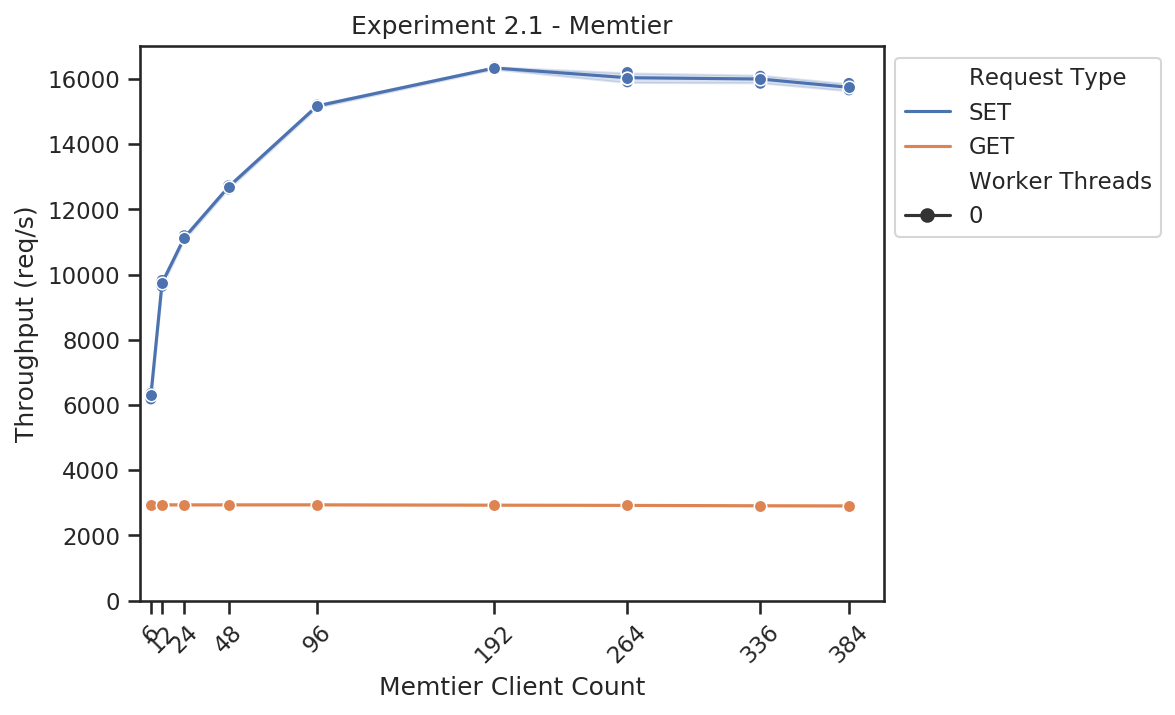
\includegraphics[width=\textwidth]{../data_analysis/figures/2-1_mt_throughput.png}
                \caption{Measured throughput on memtier.\label{fig:21_mt_tp}}
                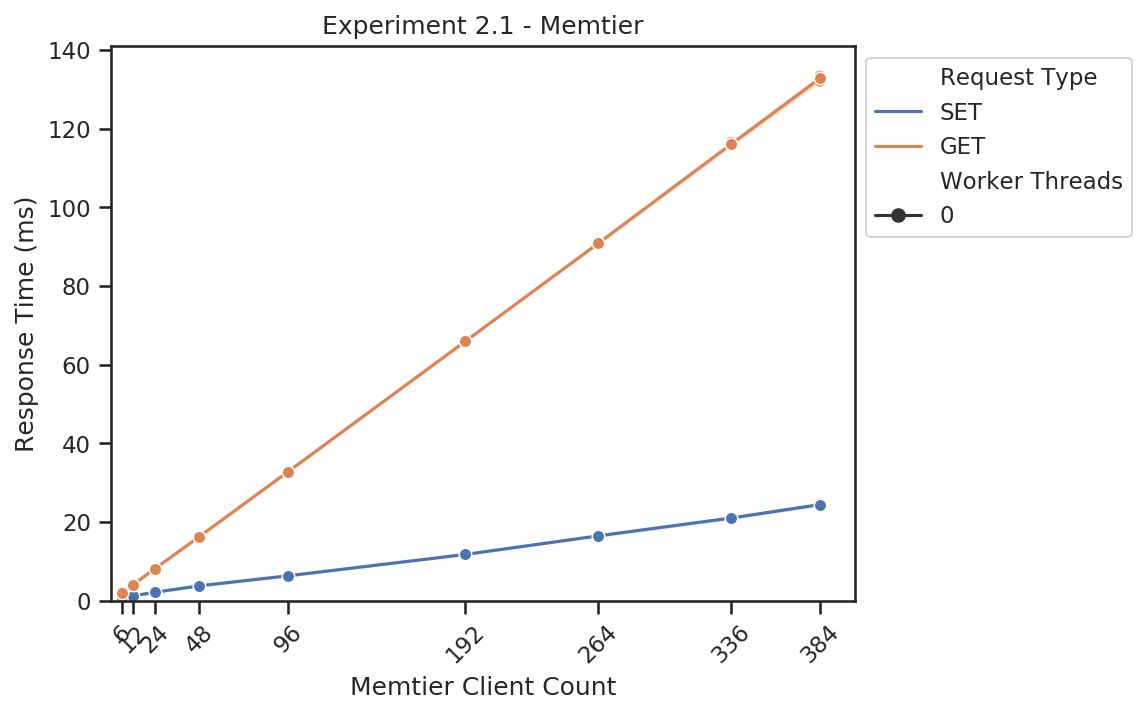
\includegraphics[width=\textwidth]{../data_analysis/figures/2-1_mt_response_time.png}
                \caption{Measured response time on memtier.\label{fig:21_mt_rt}}
            \end{subfigure}
            \begin{subfigure}[t!]{0.45\textwidth}
                \centering
                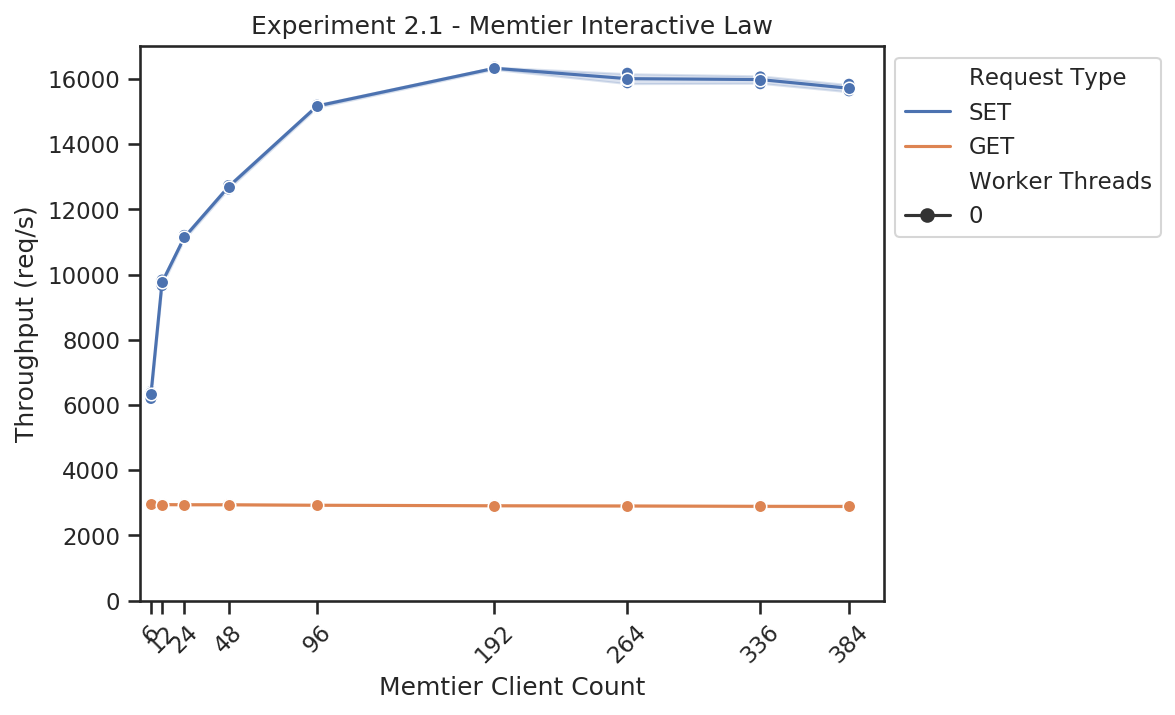
\includegraphics[width=\textwidth]{../data_analysis/figures/2-1_mt_throughput-il.png}
                \caption{Interactive Law \textendash{} Throughput.\label{fig:21_mt_tp_il}}
                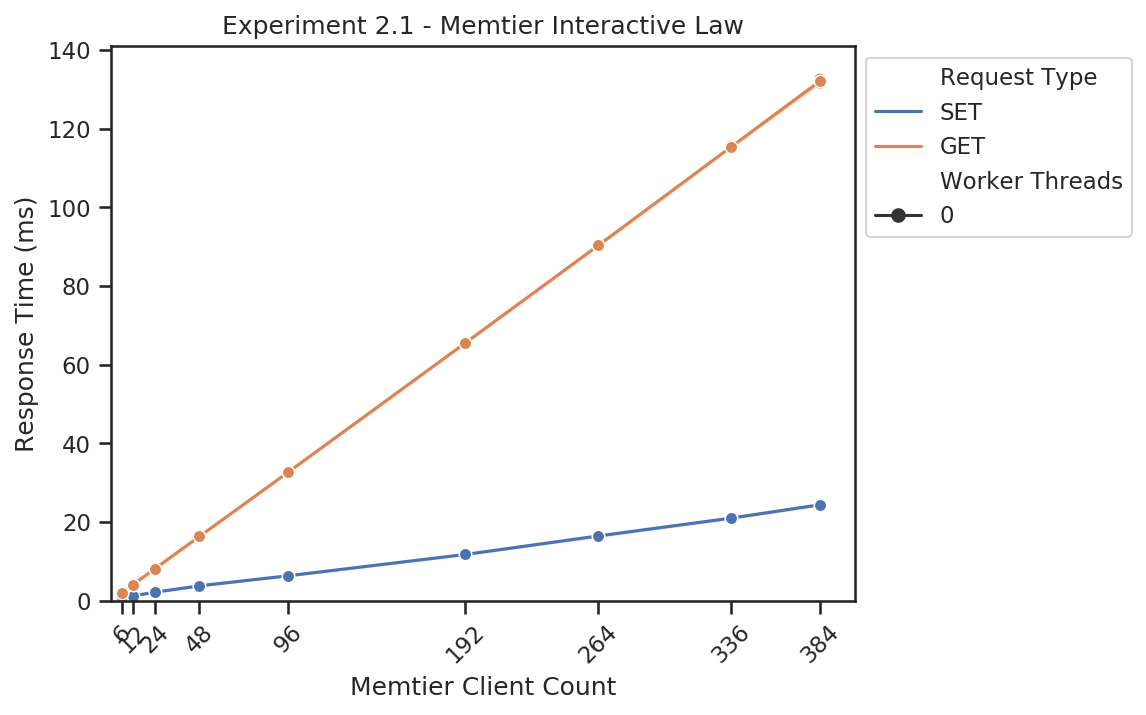
\includegraphics[width=\textwidth]{../data_analysis/figures/2-1_mt_response-time-il.png}
                \caption{Interactive Law \textendash{} Response Time.\label{fig:21_mt_rt_il}}
            \end{subfigure}
            \caption{Memtier measurements for Experiment 2.1. Error bars are plotted but not visible due to being too
                     small.}
            \label{fig:21_all}
        \end{figure*}

        \subsubsection{Explanation}

            The memcached server is from the start saturated for GET requests as increasing the amount of
            clients results in no gain of throughput. This behaviour is predicted by table \ref{tab:iperf_results}
            where the theoretical limit is 3055 requests. As such the phase of under-saturation is not observed. The
            system is at the very least saturated.  With the aforementioned 3055 requests a response time of 1.96ms
            is expected for 6 clients. The measured data of 2.04ms [0.00] indicates a good degree of saturation but
            a clear statement as to how saturated is not possible. Including the response time graph it becomes
            clear that the system is still capable of handling more participants but the respective clients will
            have slower response times.

            The memcached server behaves differently for SET requests. From a visual observation it seems to only
            saturate at 192 clients with a throughput of roughly 16000 requests\textemdash performance degrades
            thereafter. Response times scale for all points linearly and slowly; the system behaves well within
            parameters and can still handle more clients. The throughput is trending down though for very many clients
            and as such clients can expect slower response times from the system which reflect in smaller request
            throughput. It is noteworthy to mention that for SET the theoretical limit has not been reached.

            The interactive law holds as seen in figures \ref{fig:21_mt_tp_il} and \ref{fig:21_mt_rt_il}.

            We conclude therefore that the bottleneck for memcached machines is the upload of data. The next
            experiment will clarify the bottleneck for memtier machines.

    \subsection{Two Servers\label{subsec:2_two-servers}}

        \begin{figure*}
            \vspace*{-.5\baselineskip}
                \centering
            \begin{subfigure}[t!]{0.45\textwidth}
                \centering
                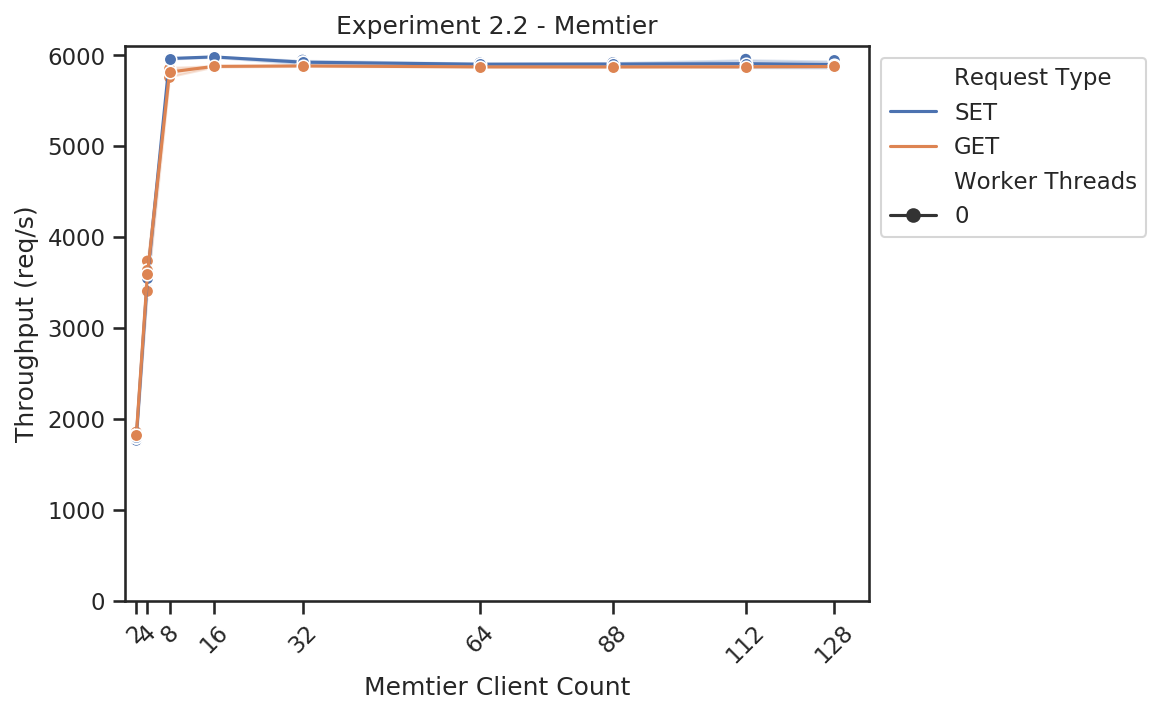
\includegraphics[width=\textwidth]{../data_analysis/figures/2-2_mt_throughput.png}
                \caption{Measured throughput on memtier.\label{fig:22_mt_tp}}
                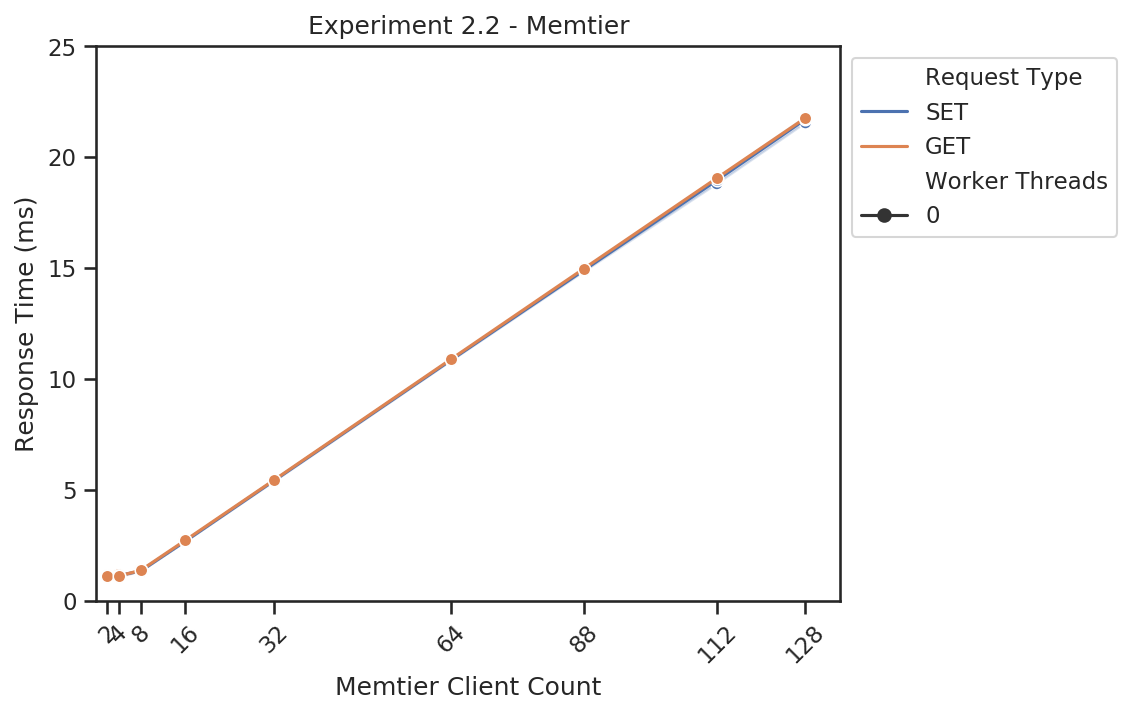
\includegraphics[width=\textwidth]{../data_analysis/figures/2-2_mt_response_time.png}
                \caption{Measured response time on memtier.\label{fig:22_mt_rt}}
            \end{subfigure}
            \begin{subfigure}[t!]{0.45\textwidth}
                \centering
                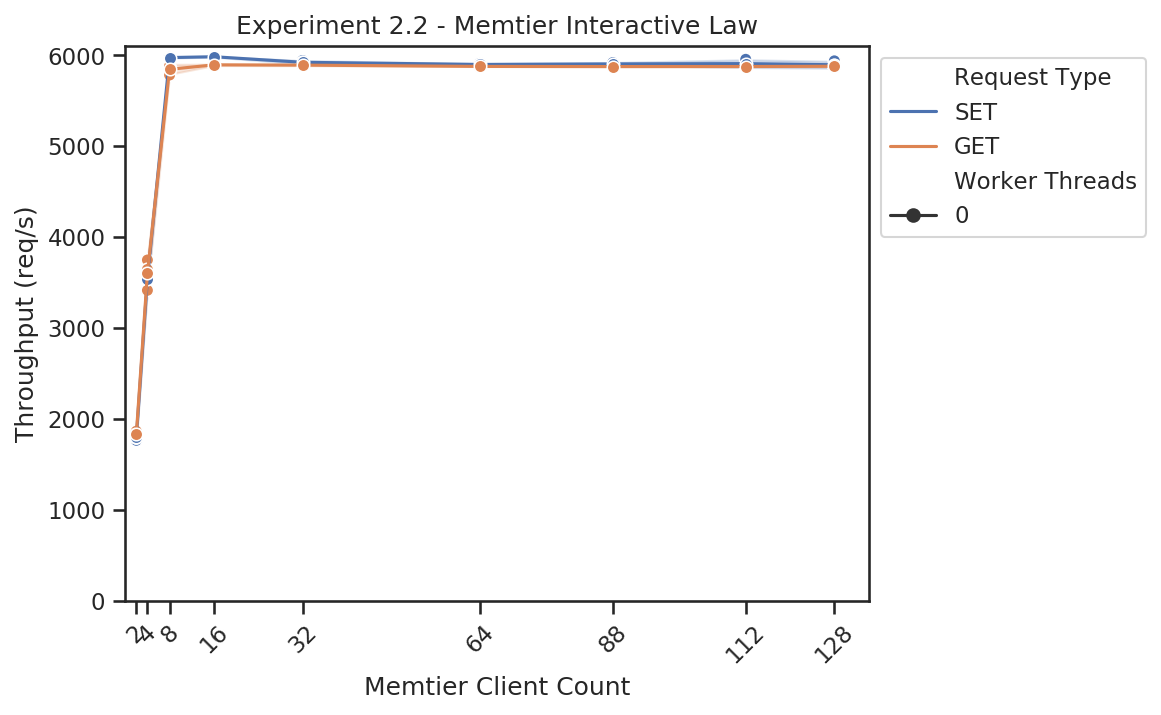
\includegraphics[width=\textwidth]{../data_analysis/figures/2-2_mt_throughput-il.png}
                \caption{Interactive Law \textendash{} Throughput.\label{fig:22_mt_tp_il}}
                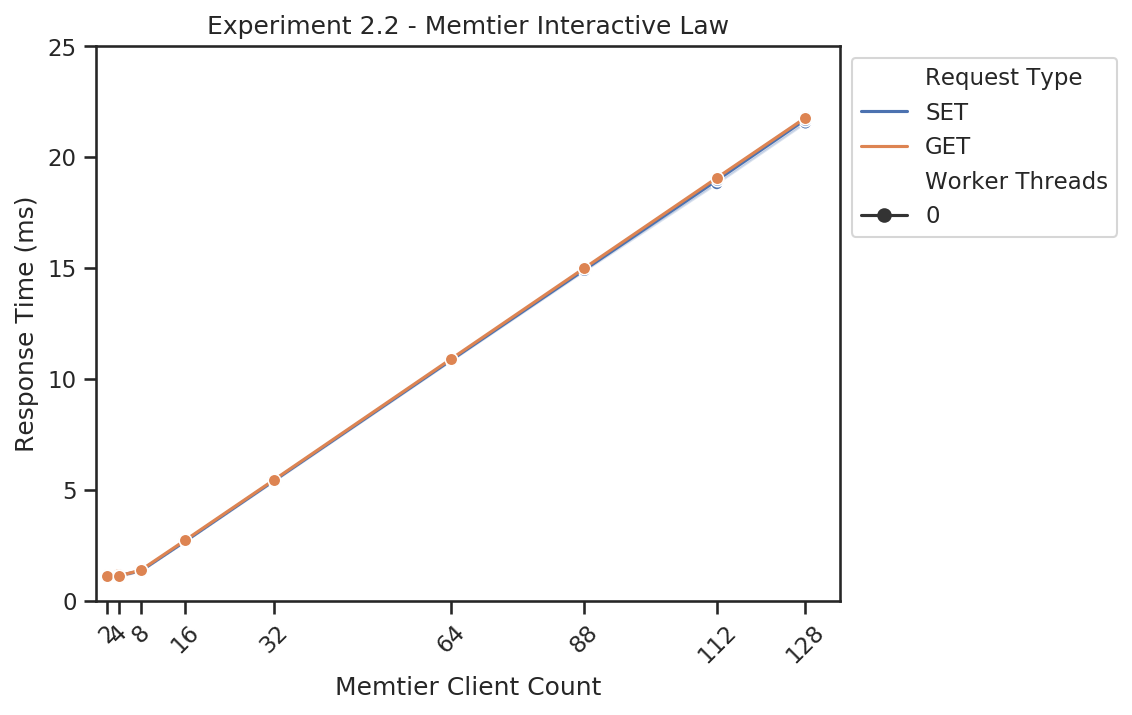
\includegraphics[width=\textwidth]{../data_analysis/figures/2-2_mt_response-time-il.png}
                \caption{Interactive Law \textendash{} Response Time.\label{fig:22_mt_rt_il}}
            \end{subfigure}
            \caption{Memtier measurements for Experiment 2.2. Error bars are plotted but not visible due to being too
                     small.\label{fig:21_all}}
        \end{figure*}

        \subsubsection{Explanation}

            The throughput of the system behaves as expected when adding another \emph{Server} to the configuration
            and removing two \emph{Client}s. SETs are reaching the network bound (cf. table \ref{tab:iperf_results})
            as more \emph{Server}s exist which allow handling twice the amount of requests for the same instance of
            time whereas GET requests also show being limited by the upload bandwidth of both \emph{Server}s (cf.
            table \ref{tab:iperf_results}). After reaching the saturation points in throughput a measurable increase
            in latency can be seen for either request type. These behaviours align with expected behaviour and also
            reflect well when applying the interactive law (figures \ref{fig:21_mt_tp_il} and
            \ref{fig:21_mt_rt_il}).

            We conclude the bottleneck for \emph{Client}s is not immediately reached but very early on. With eight
            clients being the point of saturation for GET requests for two memcached servers it is natural to assume
            that four clients are saturating one memcached server. As such the assumption of memcached being already
            over-saturated in experiment \ref{subsec:2_one-server} can be drawn.

            Memtier machines have a maximum throughput of about 5800 requests per second in these experiments. Of
            note is that the throughput doesn't compare to the previous experiment linearly but can be explained by
            a variation due to network latencies and also multiple machines resulting in overlaps of commands to
            memcached whereby some waiting is required for near-simultaneous requests as each memcached instance is run
            single-threaded.

    \subsection{Summary\label{subsec:23_summary}}

        The maximum throughput is easy to find out by visual inspection of the graphs for GET requests (as no gain
        in throughput is observed after a certain point). SET requests have for the case of three \cli{}s and one
        \srv{} more ambiguous result. One can simply look for the maximum amount of requests through the system but
        not including the increasing response time would be naive. With the limited details the decision of maximum
        saturation is a combination of limited growth in throughput and still constant growth of response times. For
        the case of one \cli{} and two \srv{}s a visual inspection is sufficient.

        \begin{table}
            \small{
                \centering
                \captionsetup{justification=centering}
                \ra{1.1}
                \begin{tabular}{@{}llll@{}}
                    \toprule
                    \textbf{Experiment} & \textbf{Read-only workload} & \textbf{Write-only workload} &
                    \textbf{Configuration} \\
                    \midrule
                    One \srv & 2637.75 [5.04]     & 16334.11 [35.27]    & Clients = 6 / 192 \\
                    One \cli & 5816.28 [51.58]    & 5965.34 [5.92]      & Clients = 8 \\
                    \bottomrule
                \end{tabular}
                \caption{Evaluation of maximum throughputs of baseline experiment. In square brackets the standard
                deviation is given, numbers are rounded to two significant figures.\label{tab:21_throughput}}
            }
        \end{table}

        The difference of how GETs and SETs are bottlenecked has been described in subsections \ref{subsec:2_one-server}
        and \ref{subsec:2_two-servers} and expected at this point. Table \ref{tab:iperf_results} summarises the
        theoretical limits.

        For the case of GET with one memcached instance this limit matches with the observed result. For two
        memcached instances with a single memtier instance this limit is twice as high as two instances are queried.
        That experiment's respective SET behaviour can be explained by the upload limit of the respective machine (cf.
        table \ref{tab:iperf_results}) and not by memcached. This claim is strengthened by the fact that a single
        instance can handle up to 16334 writes in our experiments.

        In either case for the single memtier instance, an increase in steepness for the response time can be
        observed after the saturation point. The alignment of response times for both request types matches their
        respective throughput.

        As the theoretical limit for three memtier instances should be 18233 keys it is interesting to observe only
        a utilisation of 89\%. Observing dstat results shows the system reaching full saturation on the CPU end for
        counts of 192 clients and beyond (in those cases the system is actually overloaded), meaning even though the
        network still can accommodate requests the system is CPU bound. As such it is concluded that a single \srv{}
        cannot handle more than 192 clients reasonably.

        The interactive law graphs align in all cases with the measured numbers and as such it can be deduced the
        thinking time is very close to 0 and all components introducing long response times are observable within this
        configuration.
